\xpartbox{Conclusion}

\begin{xpsectionbox}{}{}

In a disaster, this system can help provide reassurance, facilitate family reunification, enhance coordination with disaster-responding NGOs, and alleviate some of the workload on public-health personnel and other responders who interact with the community.
\newline

\noindent This project, conducted by CEB, is one of several undertaken by the NLM to address emergency conditions in the event of a disaster. Along with the National Institutes of Health's Clinical Center, the National Naval Medical Center, and Suburban Hospital, NLM is a participant in the Bethesda Hospital Emergency Preparedness Partnership (BHEPP), under whose auspices these projects are conducted.

%\begin{minipage}{0.4\linewidth}
%
%\begin{itemize}
%	  \item low-level image features (Haar, LBP, etc.)
%	  \item high-level facial landmarks (eye(s), nose, mouth, ear(s), chin, etc.)
%	  \item skin color
%\end{itemize}
%\end{minipage}
%\begin{minipage}{0.6\linewidth}
%
%\begin{center}
%%			%\hspace{-5cm}
%%			\vspace{-1cm}
%			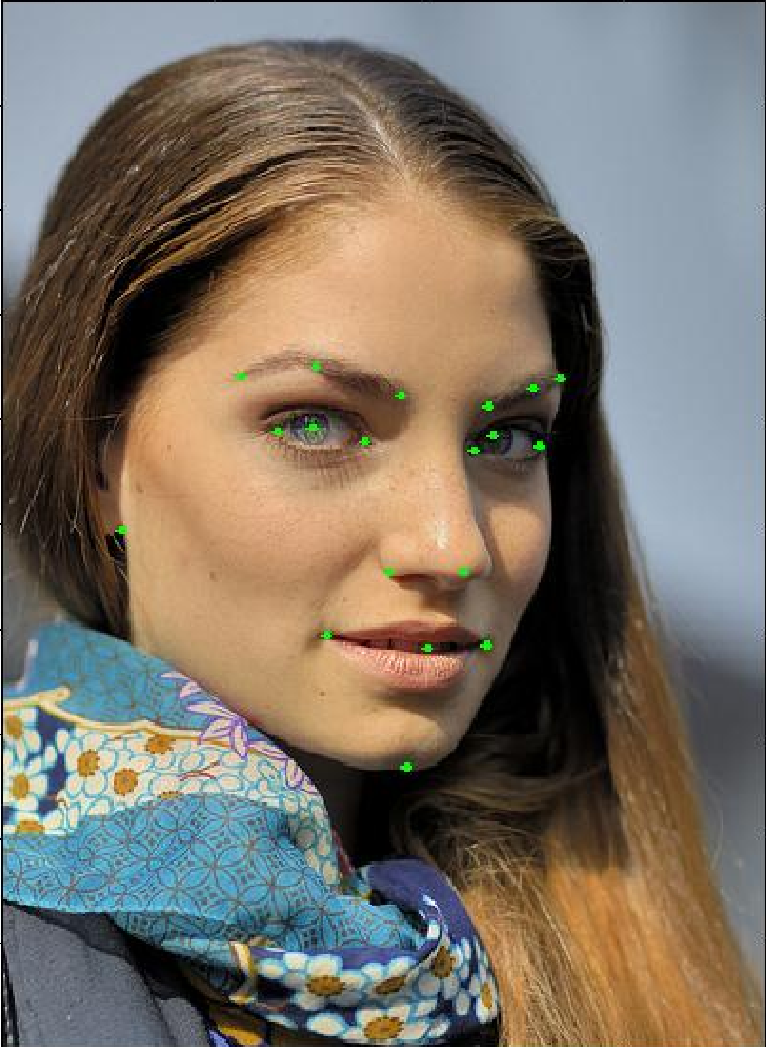
\includegraphics[height=0.25\linewidth]{images/facial_landmarks}
%			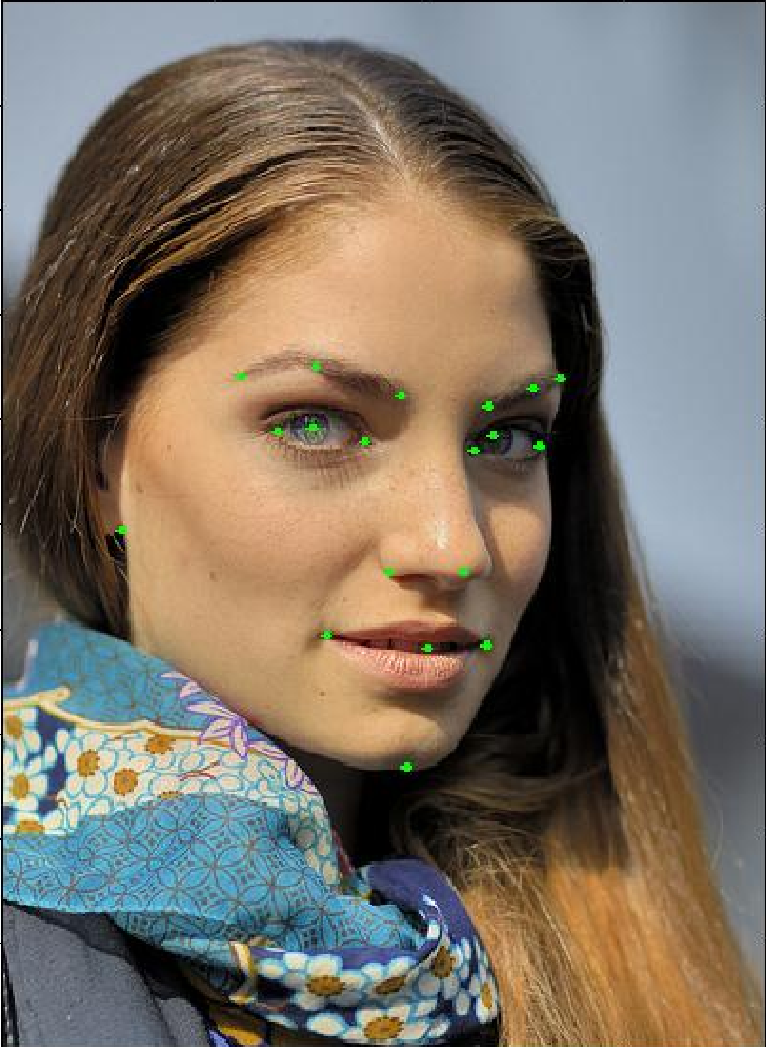
\includegraphics[height=0.25\linewidth]{images/facial_landmarks}
%\end{center}
%
%\end{minipage}
\end{xpsectionbox}



